\documentclass[10pt, a4paper]{report}
\usepackage[utf8]{inputenc}
\usepackage[T1]{fontenc}
\usepackage{amsmath}
\usepackage{amsfonts}
\usepackage{amssymb}
\usepackage{graphicx}
\usepackage{siunitx} % Provides the \SI{}{} and \si{} command for typesetting SI units
\usepackage{gensymb} % Degree symbol

\usepackage{hyperref}
\hypersetup{
	colorlinks=true,
	linkcolor=blue,
	filecolor=magenta,      
	urlcolor=cyan,
}

\author{Pranav Gade\thanks{notes from lectures by Dr. Somesh Kumar}}
\date{Dec. 2020 - Mar. 2020}
\title{Fundamentals of Electronic Engineering}


\begin{document}
	\maketitle
	\section*{Links}
	\begin{itemize}
		\item Email: \href{somesh@iiitl.ac.in}{somesh@iiitl.ac.in}
		\item Google Classroom: \href{https://classroom.google.com/u/3/c/MjQxNjk2NDYzMjc3}{https://classroom.google.com/u/3/c/MjQxNjk2NDYzMjc3}
	\end{itemize}
	\newpage
	
%	\chapter{Write the procedure to conduct the simulation in LTSpice/Circuit Lab}
%	Title:
%	Aim: To study the 
%	Component Requirements: The softwares, a computer
%	Theory: What is LTSPICE? its use, and what we can do? what are its limitations?
%	Procedure: How we can perform experiment in LTSPICE? \\
%	Open software; select resistor/copmponents; connect components; connect power supply; run/simulate
	\chapter{Introduction}	
	\section{Basic Terms}
	\begin{itemize}
		\item Thermal Voltage($V_t$): Volt equivalent of temperature $ V_t = \frac{\overline{k}T}{q} $ \\
		where\\ $\overline{k} =$  Boltzman's Constant$ = 1.381\times 10^{-23}J/\degree K  = q \times K$; \\
		$ k = 8.65 \times 10^{-5} eV/ \degree K $\\
		$ V_T = \frac{T}{11600} V$ \\
		Suppose $ T=300 \degree K $(room temp.) So, $ V_T = \frac{300}{11600} = 0.0258V = 26mV$
		\item Electron Volt(eV): Energy gained by an electron while moving through a potential difference of 1 volt. \\
		$ 1 eV = q \times P.D. = 1.69 \times 10^{-19}C \times  1V = 1.69 \times 10^{-19}CV= 1.69 \times 10^{-19}J  $(this is K.E.)
		\item Leakage Current($ I_0 $): \begin{itemize}
			\item (aka Thermally generated current) 
			\item This depends on minority Charge carrier.
			\item Never depends on applied voltage. Depends on temperature.
			\item Should be as small as possible for efficiency.
		\item\begin{tabular}{|c|c|c|}
			\hline
			& Ge & Si \\
			\hline
			$I_0$ & $\mu$A & $\eta$A \\
			\hline
		\end{tabular}
			\item Small leakage current -> no false triggering(randomly turning on)
			\item Therefore, Si is better because no false triggering.
			\item $ I_{0(T_0)}  = I_{0(T_1)}  \times  2^{\frac{T_2 - T_1}{10}}$
			\item $ I_0 $ will double every 10\degree C rise in temp(for Si, Ge)
			\item $ I_0 $ is 7\% higher for 1\degree C rise in temp.
			\item Si is better for high temp because smaller $ I_0 $, which can eliminate false triggering.
		\end{itemize}
		\item Energy Gap($ E_g $):\begin{itemize}
			\item aka Band Gap, see fig. \ref{fig:energy-band-diagram}
			\begin{figure}
				\centering
				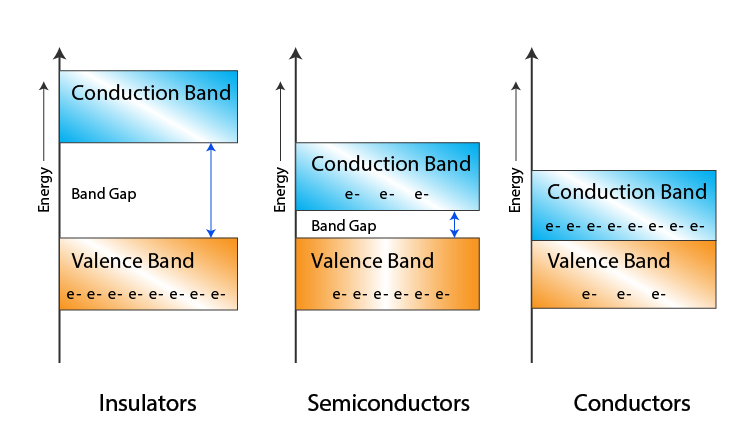
\includegraphics[width=0.7\linewidth]{img/Energy-band-diagram}
				\caption[Energy Bands]{Energy Bands}
				\label{fig:energy-band-diagram}
			\end{figure}
			
			\item Metals: $ E_g = 0 $ even at 0K. So, $ e^- $ are available even at 0K.
			\item Semiconductor: At 0K, behaves like insulator($ E_g = 1eV $). At 300K, band gap starts decreasing so conductivity increase.
			\item Insulator: $ E_g = 5eV \;to\; 15 e $ so $ e^- $ will not jump at any temp.
			\item $ E_g \propto \dfrac{1}{temp} $
			\item $ E_{g(T)} = E_{g0} - \beta T $; ($\beta$ is $ 2.2  \times  10^{-4} $ for Ge; $ 3.6 \times  10^{-4} $ for Si)
			\item \begin{tabular}{|c|c|c|c|}
				\hline
				& Ge & Si & GaAs \\
				\hline
				$ E_{g0} $ & 0.75eV & 1.21eV & - \\
				\hline
				$ E_{g300} $ & 0.72eV & 1.1eV & 1.47eV \\
				\hline
			\end{tabular}
		\end{itemize}
	\end{itemize}
		
\end{document}